% -*- latex -*-
%%%%%%%%%%%%%%%%%%%%%%%%%%%%%%%%%%%%%%%%%%%%%%%%%%%%%%%%%%%%%%%%
%%%%%%%%%%%%%%%%%%%%%%%%%%%%%%%%%%%%%%%%%%%%%%%%%%%%%%%%%%%%%%%%
%%%%
%%%% This text file is part of the source of 
%%%% `Introduction to High-Performance Scientific Computing'
%%%% by Victor Eijkhout, copyright 2012-2021
%%%%
%%%% This book is distributed under a Creative Commons Attribution 3.0
%%%% Unported (CC BY 3.0) license and made possible by funding from
%%%% The Saylor Foundation \url{http://www.saylor.org}.
%%%%
%%%% listing.tex : demo of the LaTeX listings package
%%%%
%%%%%%%%%%%%%%%%%%%%%%%%%%%%%%%%%%%%%%%%%%%%%%%%%%%%%%%%%%%%%%%%
%%%%%%%%%%%%%%%%%%%%%%%%%%%%%%%%%%%%%%%%%%%%%%%%%%%%%%%%%%%%%%%%

\documentclass{artikel3}

\usepackage[pdftex]{hyperref}
\usepackage{pslatex}

\usepackage{wrapfig}
\usepackage{pgfplots}  
\pgfplotsset{width=6.6cm,compat=1.7}  

\usepackage{geometry}
\addtolength{\textwidth}{.75in}
\addtolength{\textheight}{.75in}

\begin{document}
\title{SSC 335: barchart demo}
\author{Victor Eijkhout}
\date{today}
\maketitle

\section{Two graphs}

\begin{wrapfigure}{l}{2in}
  \hrule width 3in height 0pt
  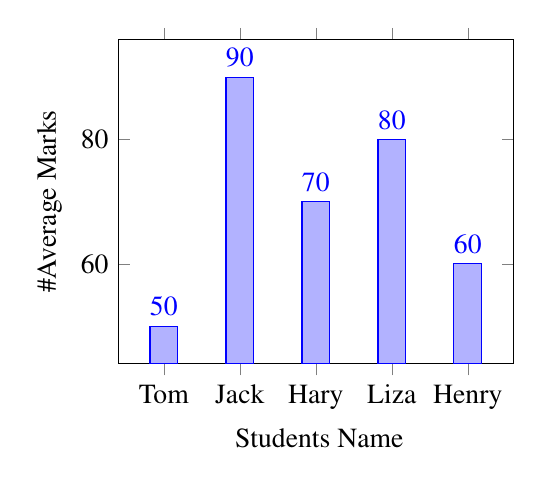
\begin{tikzpicture}  
    \begin{axis}  
      [  
        ybar,  
        enlargelimits=0.15,  
        ylabel={\#Average Marks},
        xlabel={\ Students Name},  
        symbolic x coords={Tom, Jack, Hary, Liza, Henry},
        xtick=data,  
        nodes near coords,
        nodes near coords align={vertical},  
      ]  
      \addplot coordinates {(Tom,50) (Jack,90) (Hary,70) (Liza,80) (Henry,60) };  
    \end{axis}  
  \end{tikzpicture}
\end{wrapfigure}
Lorem ipsum dolor sit amet, consectetur adipiscing elit, sed do eiusmod tempor incididunt ut labore et dolore magna aliqua. Pharetra massa massa ultricies mi quis hendrerit. Tempor nec feugiat nisl pretium fusce id velit ut tortor. Eget nulla facilisi etiam dignissim diam quis enim. Cursus sit amet dictum sit amet justo donec. Tortor consequat id porta nibh venenatis cras sed felis eget. Senectus et netus et malesuada fames ac turpis egestas integer. Ultricies mi quis hendrerit dolor magna eget est. A iaculis at erat pellentesque adipiscing. Sagittis orci a scelerisque purus. Quisque non tellus orci ac. Nisl nunc mi ipsum faucibus. Vivamus at augue eget arcu dictum varius duis. Maecenas ultricies mi eget mauris pharetra et ultrices neque ornare. Pulvinar neque laoreet suspendisse interdum consectetur. Nunc id cursus metus aliquam eleifend mi. Tristique sollicitudin nibh sit amet commodo nulla. Massa tincidunt nunc pulvinar sapien et ligula ullamcorper malesuada. Justo laoreet sit amet cursus sit. Laoreet id donec ultrices tincidunt arcu non sodales.

\begin{wrapfigure}{r}{2in}
  \hrule width 3in height 0pt % kludge: picture is not wide enough
  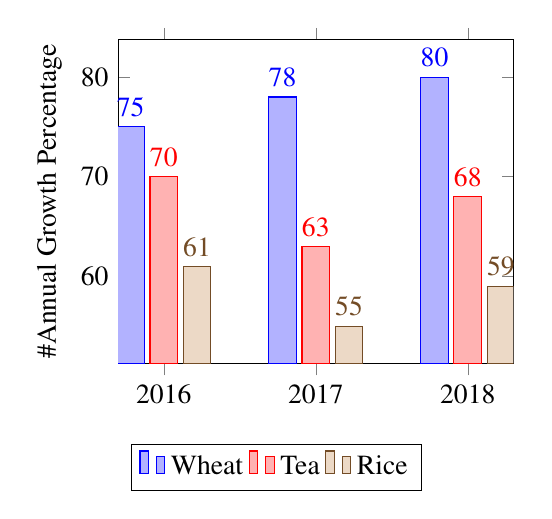
\begin{tikzpicture}  
    \begin{axis}  
      [  
        ybar,
        enlargelimits=0.15,
        legend style={at={(0.4,-0.25)},anchor=north,legend columns=-1},     
        ylabel={\#Annual Growth Percentage},
        symbolic x coords={2016, 2017, 2018},  
        xtick=data,  
        nodes near coords,  
        nodes near coords align={vertical},  
      ]  
      \addplot coordinates {(2016, 75) (2017, 78) (2018, 80)};
      \addplot coordinates {(2016, 70) (2017, 63) (2018, 68)};  
      \addplot coordinates {(2016, 61) (2017, 55) (2018, 59)};  
      \legend{Wheat, Tea, Rice}  
    \end{axis}  
  \end{tikzpicture}  
\end{wrapfigure}
Sem nulla pharetra diam sit amet. Vel pharetra vel turpis nunc eget. Vulputate dignissim suspendisse in est ante in nibh mauris cursus. Sem viverra aliquet eget sit amet tellus cras. Rhoncus aenean vel elit scelerisque mauris pellentesque pulvinar pellentesque. Fusce ut placerat orci nulla pellentesque. Vel risus commodo viverra maecenas accumsan lacus vel facilisis volutpat. Enim ut tellus elementum sagittis vitae et. In nibh mauris cursus mattis molestie. Curabitur gravida arcu ac tortor dignissim convallis aenean et tortor. Mauris commodo quis imperdiet massa.

\end{document}
